\chapter{Design} \label{cha:design}
	This chapter explains the design of the system. This includes: back-end
	design, model/graphical design, and main activities.

	\section{Main activities} \label{sec:mainactivities}
		There are several main activities in the system, corresponding to the two
		main user types of the system. These user types are both the physically co-
		located	players as well as the physically remote players. The activities
		are as follows:

		\subsection{A local user wants to start a game} \label{ssec:userstartgame}
			The local user ensures the main camera is set up according to the 
			provided guidelines. The local user then starts the server on the 
			machine the camera is connected to. The local user needs to take note 
			of the IP address of the server machine and fill this into his local 
			machine (to which the Meta One glasses are attached). The other players
			also fill in the same IP address. The server can also run on one of the 
			players' machines. The local user needs to wait for others to join the 
			game. When at least two local players and at least one remote player 
			has joined the game, the game will start.
			
		\subsection{A local user wants to join a game} \label{ssec:localjoingame}
			A local player wants to join an active game. Before this can
			happen, a game has to be started first. The local player needs to 
			acquire the IP address of the server machine and fill this in.
			Once the game starts, the local player will see virtual objects projected 
			through the Meta One glasses.

		\subsection{A remote user wants to join a game} \label{ssec:remotejoingame}
			A physically remote player wants to join an active game. Before this can
			happen, a game has to be started first. The remote user needs to acquire 
			the IP address of the local server machine (see \ref{ssec:userstartgame})
			and fill this in. The remote user will see a virtualized version of the 
			same game world as the local players.
			
		\subsection{A local player wants to move a mirror} \label{ssec:localmovemirror}
			A local player is partaking in an active game. To hit the target, they
			need to move a mirror from point A to point B to allow the laser beam
			coming from the emitter to be deflected and therefore to hit the target.
			The local player uses moveable markers to place a mirror in the game
			world. Using the Meta One glasses, local players can see the game objects
			when they see a marker. For this example, it is assumed that the player that wants
			to move the mirror marker also has that mirror marker to their disposal,
			and also that the mirror is rotated such that no more rotation is required.
			The local player can then take the mirror marker, move it to the point
			it should be moved to, and complete the game that way.
			
		\subsection{Two local players want to move a mirror} \label{ssec:localmovemirrorcollab}
			Due to mirror markers being divided between the players, it is possible
			that two (or, more generally speaking, multiple) players want to move
			a mirror, possibly the last mirror required to solve the level. However,
			a mirror marker can only be placed by one person. The local players then
			need to collaborate on where the marker should be placed. As the players
			are physically co-located (by definition of them being local players),
			this collaboration can happen in multiple ways, like pointing to a 
			location on the playing field, or discussing the best position for the
			marker.
			
		\subsection{A remote player wants to rotate a mirror} \label{ssec:remoterotatemirror}
			Remote players, due to them not being physically co-located with the
			local players, cannot move mirror markers, as that would require them
			to meet up with the local players and to play with them. However, 
			remote players have access to an ability that the local players do
			not have access to, that being the ability to rotate selected mirrors.
			The remote player uses a computer for this. In order to rotate a mirror,
			the player has select a mirror first. Using the "M" key, the player can
			cycle through mirrors, but they can also click on a mirror in the game
			world to select that mirror. When a mirror is selected, the outer
			frame of the mirror (shown in \ref{fig:mirror}) will change color
			from gold to bright yellow, indicating that this mirror is selected
			(the recolor will only be visible for the remote player responsible
			for clicking on that mirror, even other remote players will not be
			able to see this recolor). Also, a selected mirror can be rotated by
			using the "A" key (for rotation to the left, relative to the surface
			normal of the mirror) or the "D" key (for rotation to the right).
		
		\subsection{Use case diagrams} \label{ssec:usecasediagrams}
			To illustrate the given main activities, two use case diagrams are
			displayed here. The use cases for the remote player are depicted in
			\ref{fig:remoteusecase}, while the use cases for the local player
			are depicted in \ref{fig:localusecase}.
			\begin{figure}[!ht]
				\centering
				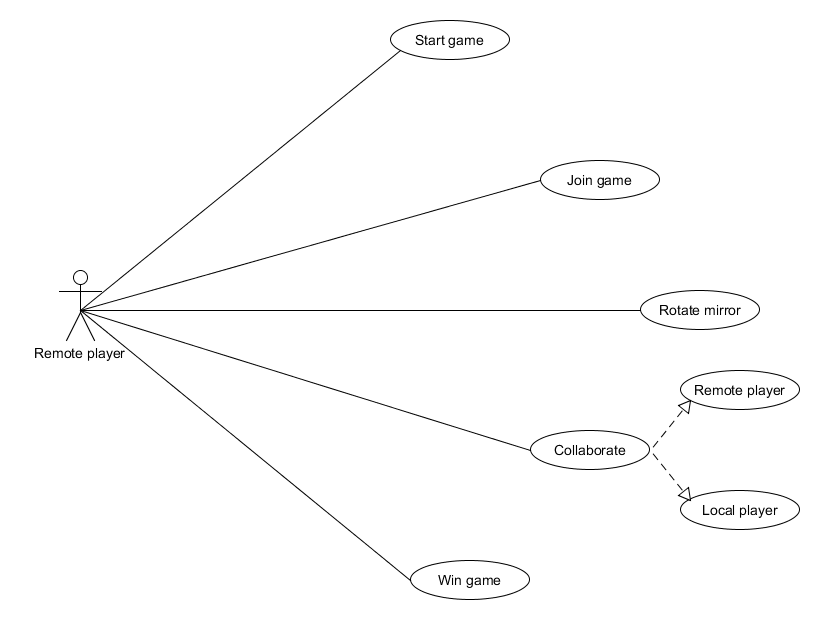
\includegraphics[scale = 0.4]{RemotePlayerUseCase}
				\caption{The use cases for the remote player.}
				\label{fig:remoteusecase}
			\end{figure}
			\begin{figure}[!ht]
				\centering
				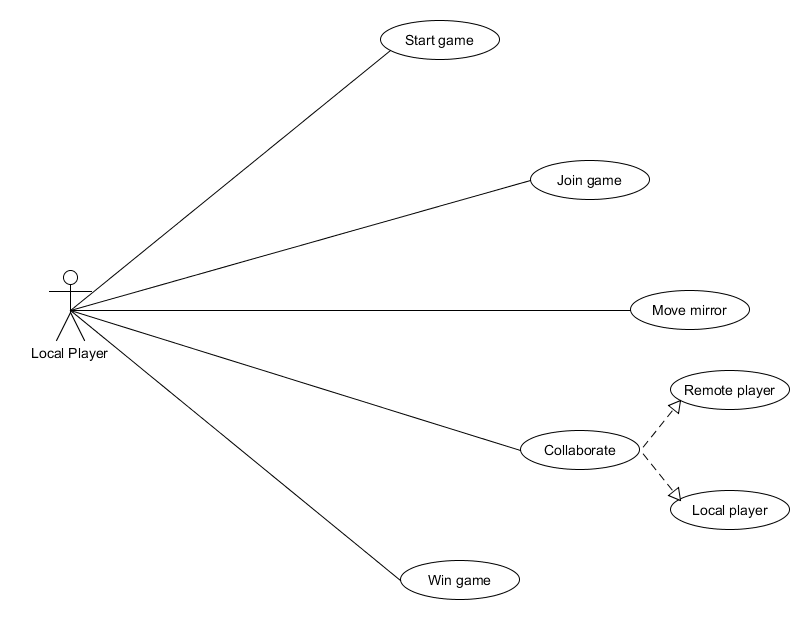
\includegraphics[scale = 0.4]{LocalPlayerUseCase}
				\caption{The use cases for the local player.}
				\label{fig:localusecase}
			\end{figure}
		%TODO add some use case diagrams?

	\section{Back-end design} \label{sec:backenddesign}
		The system is composed of three main parts: The Laser mechanics, the network
		functionality and the projection to 3D glasses. For this purpose, we divided
		the C\# code over three namespaces, named "Core", "Network" and
		"Projection", respectively.

		The "Core" namespace is responsible for drawing the Laser beams and
		providing the interactions of laser beams with the other game objects.
		The layout of this namespace is discussed in paragraph 
		\ref{ssec:corenamespace}.

		The "Network" namespace is responsible for synchronizing the game state
		between all connected players. The layout of this namespace is discussed 
		in paragraph \ref{ssec:networknamespace}.

		The "Projection" namespace is responsible for providing the projection to
		the VR glasses. This namespace provides the functionality required to project
		the game world to the VR glasses. The layout of this namespace is discussed in
		paragraph \ref{ssec:projectionnamespace}.
		
		The "Vision" namespace is responsible for containing tracked markers.
		At first this was part of the responsibility of the "Projection"
		namespace, but that namespace got too big and needed to be split,
		resulting into this extra namespace. The layout of this namespace is
		discussed in paragraph \ref{ssec:visionnamespace}.
		
		Additionally, the game depends on the deployment of a server application
		written in C++. The purpose of this server application will be discussed 
		along with the Network namespace in \ref{ssec:networknamespace}. Also,
		in the past we wanted to potentially add random levels for replay value,
		and this is discussed in paragraph \ref{ssec:randomlevelnamespace}
		
		\subsection{The Core namespace} \label{ssec:corenamespace}
			The \texttt{Core} namespace contains all the code for all the core gameplay
			elements. The term "core gameplay elements" refers to all the
			elements necessary to play the basic game with, basically the code
			for the game objects. Using only the code from the \texttt{Core} namespace,
			it would be possible to create the same game without using AR
			technology or using markers to play the game with, for that matter.
			
			The \texttt{Core} namespace is further subdivided into three namespaces:
			the \texttt{Core} namespace itself, which contains code relating to the laser
			and code that helps the other two namespaces, the 
			\texttt{Core.Emitter} namespace, which contains code for objects 
			that emit laser beams, and the \texttt{Core.Receiver} namespace, 
			which contains code for objects that receive laser beams and have to 
			do something with these beams.
			
			There are several game objects that emit laser beams as well as 
			receive them (as seen in \ref{sec:graphicaldesign}). This causes the
			\texttt{Core.Emitter} and \texttt{Core.Receiver} namespaces to have 
			some coupling. However, the coupling is minor, and coupling is only 
			between sub-namespaces in the same main namespace. As such, this 
			should not cause that much of a problem, when considered in a 
			software engineering context.
			
			\begin{figure}[ht]
				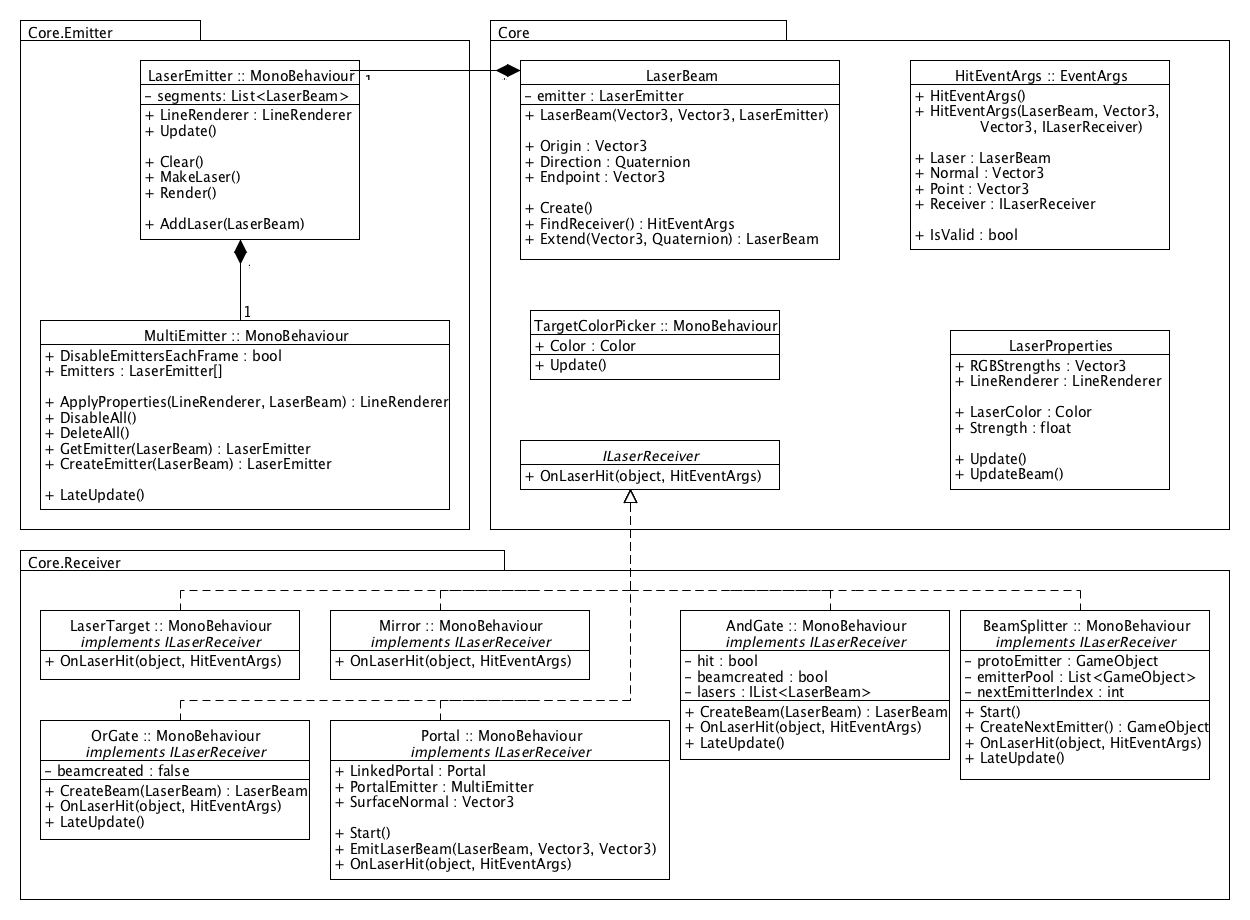
\includegraphics[width=\textwidth]{ClassDiagramCore}
				\caption{Class diagram of the \texttt{Core} namespace}
				\label{fig:classdiagramcore}
			\end{figure}
			
		\subsection{The Network namespace} \label{ssec:networknamespace}
			The \texttt{Network} namespace has undergone several changes since the start
			of the project. These changes are described in this part.
			
			The first take on creating a network functionality in the game
			was to use the standard way of networking within Unity itself.
			This involved creating a rather simple networking script that
			allowed the game to connect to the Unity master server or their own
			master server (provided they had one installed), which then handled
			all changes that were recorded by network view components of objects,
			and sent them to all the players, synchronizing the game world.
			There are several tutorials on how to write such a networking
			script and how to use it in a multiplayer game, the tutorial that
			was used for the script in the namespace can be found here:
			\url{http://www.paladinstudios.com/2013/07/10/how-to-create-an-online-multiplayer-game-with-unity/}
			
			The base networking functionality of Unity, however, was not enough
			for what we were trying to do (for example, it had very poor VR and
			AR support, and our game is an AR game after all). Because of this,
			a different solution was required to create synchronization across
			the game world. The next option was to use the Photon Unity Networking
			package, which not only supported multiplayer better (it allowed for
			more people to play the same game), but it also allowed VR and AR games
			to have multiplayer functionality (there is a free package available
			on the Unity Asset Store, which can be found here: \url{https://www.assetstore.unity3d.com/en/#!/content/1786}). However,
			this was not used, as the problem was not that we needed to connect
			several AR players in the game world (as these would be the local players,
			and therefore would be able to see what was going on in the game world
			by just looking at the marker that was placed near them). As such,
			a different solution had to be found.
			
			The final solution is the solution that is used right now. Instead of 
			relying on Unity for the networking functionality, we decided to 
			combine this problem with another issue we came across regarding 
			the detection and synchronisation of marker locations. This solution
			was to deploy a server, written in C++, that uses OpenCV to detect 
			the markers. This also allows us full control over the detection and 
			manipulation of object transformations in Unity, as this was causing 
			issues with both the Meta One SDK as well as Vuforia.
			
			The OpenCV server makes use of a single camera to detect marker locations.
			These locations are then sent to all clients over a socket connection.
			This solution makes it easier to synchronize object positions between users
			because all gameplay activities take place in a predefined area on a table,
			and the users need only look at a single marker to be able to see the 
			entire scene. 
			
			\begin{figure}[ht]
				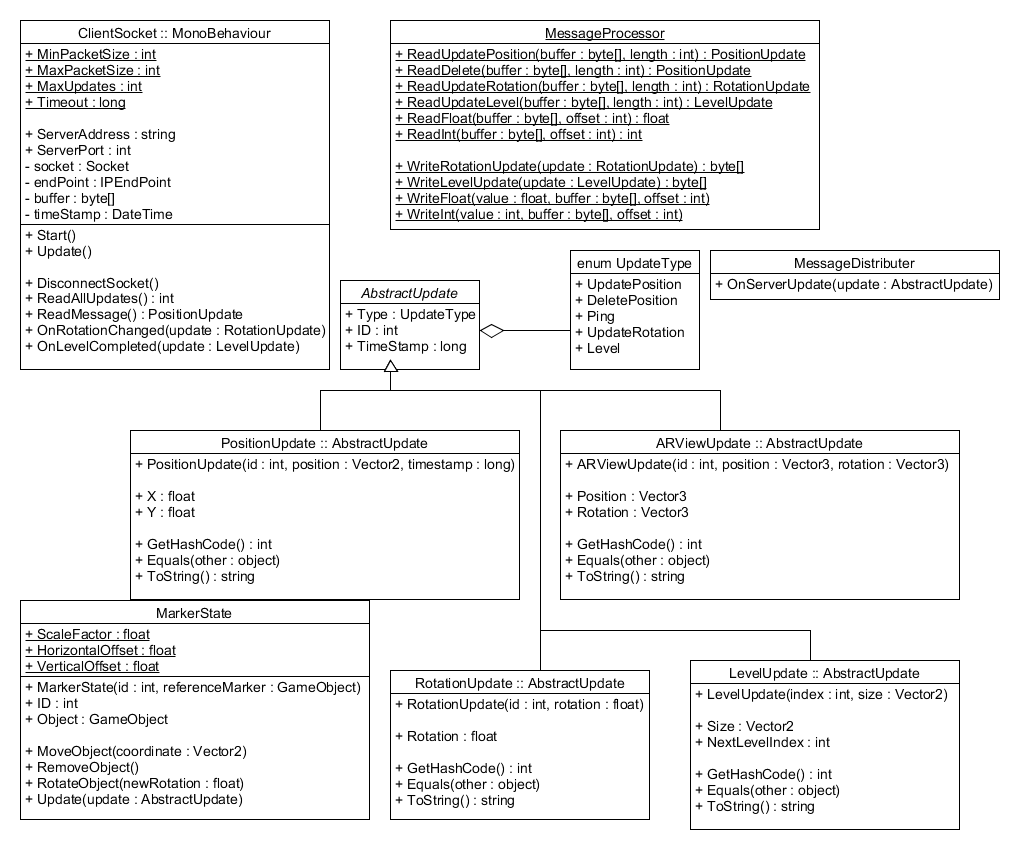
\includegraphics[width=\textwidth]{ClassDiagramNetwork}
				\caption{Class diagram of the \texttt{Network} namespace}
				\label{fig:classdiagramnetwork}
			\end{figure}
			
		\subsection{The Projection namespace} \label{ssec:projectionnamespace}
			The \texttt{Projection} namespace is responsible for projecting the 
			world to the Meta One glasses. It takes care of detecting 
			markers in the playing area and projects all objects relative
			to those markers. 
			
			The main responsibility, fixing the projection to the Meta One 
			glasses, is partly taken care of by the Meta SDK. However, the 
			Meta SDK moves and rotates all game objects to fit the actual 
			position and rotation of the Meta One. Due to the limited field 
			of vision of the Meta One glasses, not all markers can be seen at 
			the same time. In order to ensure the game objects and 
			corresponding laser beams still appear at the correct positions,
			the Network namespace provides relative positions and rotations for 
			all game markers in the playing area (also see paragraph 
			\ref{ssec:networknamespace}). The \texttt{Projection} namespace then uses
			this information to place the objects in correct positions relative
			to any marker detected by the Meta SDK. This ensures that all objects
			remain visible and in the correct locations, as long as the Meta SDK 
			tracks at least a single marker.
			
			Note that even if the marker cannot be detected temporarily, there 
			is only a slight error in the locations of objects. This is due to 
			the use of SLAM localization for tracking markers. See the paragraph
			about SLAM localization (\ref{ssec:slamloc}) for details on how SLAM 
			localization works.
			
			See figure \ref{fig:classdiagramprojection} for the class diagram for 
			the Projection namespace.
			
			\begin{figure}[ht]
				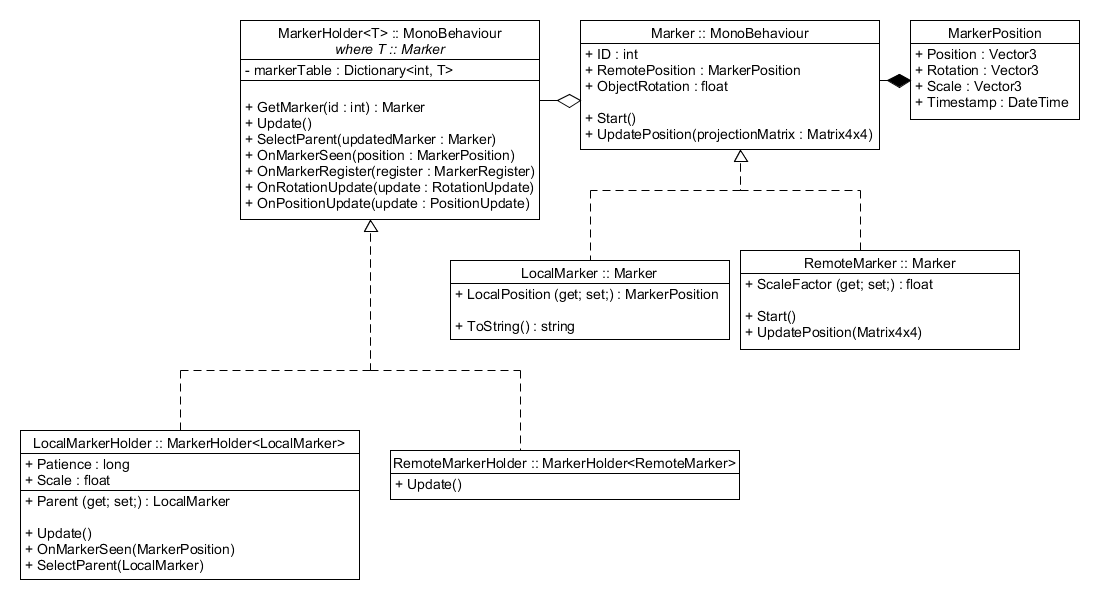
\includegraphics[width=\textwidth]{ClassDiagramProjection}
				\caption{Class diagram of the \texttt{Projection} namespace}
				\label{fig:classdiagramprojection}
			\end{figure}
			
		\subsection{The Vision namespace} \label{ssec:visionnamespace}
			The \texttt{Vision} namespace is a small namespace responsible for
			containing tracked markers and their ID's. It used to be a part
			of the \texttt{Projection} namespace, but it got split off,
			because it had little to do with fixing the projection of the
			META One, and more with containing tracked markers. Also, the
			\texttt{Projection} namespace became way too big during development
			(it started with about four to five classes, and those got split
			up into about fifteen classes, mainly because they violated software
			engineering principles such as the single responsibility principle).
			Because it got so big, some of the classes needed to be split off from
			the namespace and put into another namespace.
			
			By design, and because of how it was conceived, the \texttt{Vision} 
			namespace depends heavily on the \texttt{Projection} namespace.
			However, this dependency is not cyclic, and should not cause too
			much of a problem because of it, when viewed from a software
			engineering standpoint. The only communication from the \texttt{Vision}
			namespace to the \texttt{Projection} namespace is by sending out
			messages into the object hierarchy, which are then received by 
			components that can actually receive said messages. 
			
			\begin{figure}[ht]
				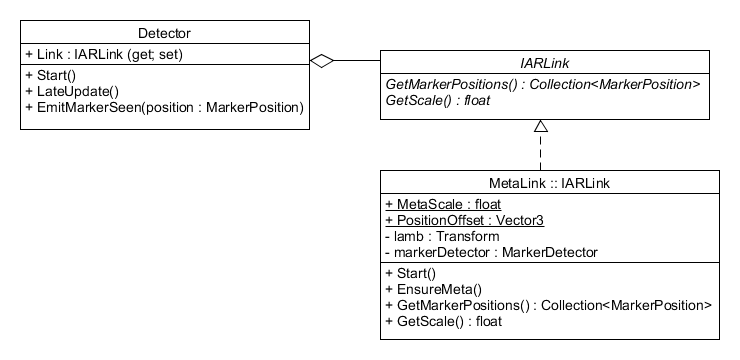
\includegraphics[width=\textwidth]{ClassDiagramVision}
				\caption{Class diagram of the \texttt{Vision} namespace}
				\label{fig:classdiagramvision}
			\end{figure}
			
		\subsection{Experimental code: the RandomLevel namespace} \label{ssec:randomlevelnamespace}
			The \texttt{RandomLevel} namespace is an abandoned and deleted
			namespace, which contained code that, when deployed, would create
			rather simple but random levels with one target and one laser.
			The levels are always solvable, and would be created according 
			to an algorithm that is explained in this section.
			
			The algorithm that was used to create random levels is as follows:
			First, a square grid of points is made. The grid was represented by
			2D array (a matrix) of grid points. Second, the laser target is
			placed in the middle of the matrix. Third, a spiral path is created that
			goes from the laser to an outer edge of the matrix. This path is then
			known as the critical path. Finally, walls are added to the level randomly,
			however they are never placed on either the target, a part of the
			critical path, or the laser. The walls are also rotated either
			horizontally or vertically. As can be seen, the levels created were
			rather simple (as they did not contain our more advanced game
			objects, only targets and walls), and solving them could always be done
			with several mirrors. The four phases of the randomization algorithm
			are displayed graphically in \ref{fig:random}. The first image depicts
			the grid, the second depicts the laser target as a red dot in the
			middle of the map, the third image depicts the spiral path that
			is created from the target (the orange dot) to the edge of the map 
			(this spiral path always bends four times, and can start in any 
			random direction), the final image depicts the random placement of
			walls as purple dots.
			
			\begin{figure}[ht]
				\centering
				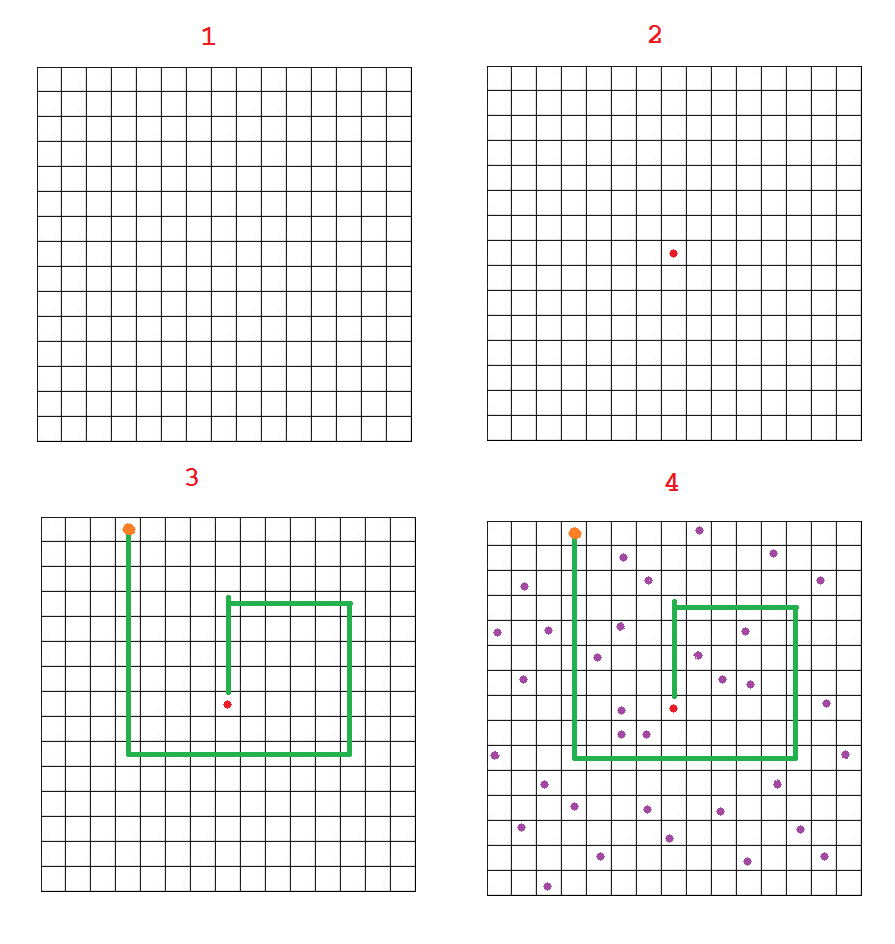
\includegraphics[scale = 0.4]{RandomLevelAlgorithm}
				\caption{The random level algorithm, displayed graphically.}
				\label{fig:random}
			\end{figure}
			
			The random level generation was added very early on in the project,
			and there was some value in developing it further (think of replay
			value for the game, for example). It was also changed later to
			allow for more possible paths (not only spirals, but also paths with
			less or more than four bends). However, it was scrapped after
			discussing it with our coach, especially after talking about how it
			would increase the replay value of the game. Another reason to abandon 
			it was because the classes belonging to it were some of the most complex
			in the project. Even after several attempts to rewrite these classes, 
			they were still just barely under the maximum complexity that we
			allowed for our classes. This was measured with SonarQube, explained
			in section \ref{cha:qa}.
			
	\section{Game elements} \label{sec:graphicaldesign}
		For designing the 3D models, we used Blender. Blender is a free 
		application for 3D modeling, under the GNU General Public License, and 
		Unity natively supports Blender models (provided it is installed on
		the system). We have chosen for a light looking style featuring nature 
		inspired models and gold and crystal based materials. The light modeling
		style causes slight misalignments with the ground to be less noticeable 
		and makes the lack of feedback from moving a card feel less odd. The 
		crystals and gold just feels good in combination with the beams of light.
		
		The following sections display and describe the graphics used in the 
		game play elements, as well as the function of these elements.
		%TODO Explain why we chose this graphics style
		
		\subsection{Laser target} \label{ssec:lasertarget}
			The laser target is the main target of the game. It consists of
			a small container, which contains a crystal. The point of the
			game is to direct a laser beam from an emitter to this target.
			When the target is hit by a laser beam, the outer columns around
			the crystal inside will rotate and spread out, indicating that
			the target has been hit. The game will proceed to the
			next level once all targets are hit. An image of the target is shown in figure 
			\ref{fig:target}. The gold columns depicted are the outer columns
			described earlier. Also, the inner crystal will change color
			when hit.
			\begin{figure}[!ht]
				\centering
				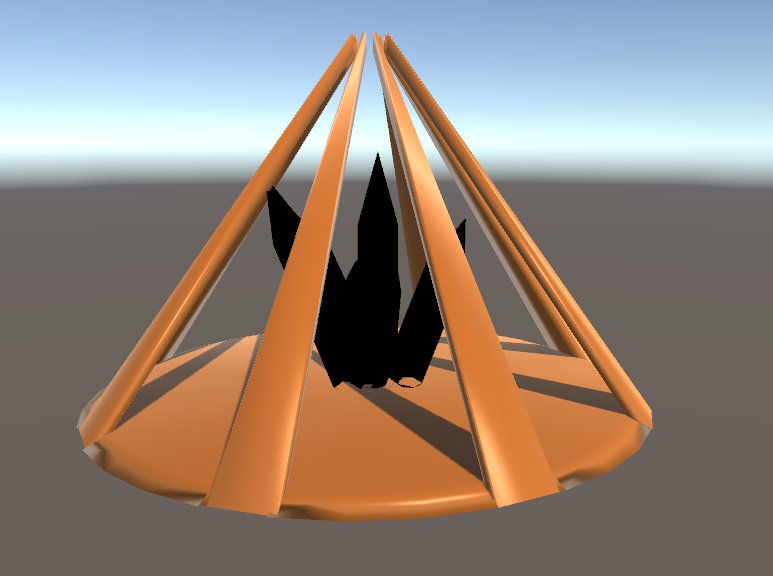
\includegraphics[scale = 0.4]{Target}
				\caption{The laser target.}
				\label{fig:target}
			\end{figure}
			
		\subsection{Mirror} \label{ssec:mirror}
			A mirror is a crucial game element. Its reflective surfaces
			allow it to reflect any laser beam that hits these surfaces.
			It is also the only element that players can move and/or rotate.
			All levels require at least one mirror to move or rotate
			in order to hit the target. An image of a mirror in-game is shown
			in \ref{fig:mirror}. The light blue circles reflect laser beams, 
			the golden outer frame does not.
			\begin{figure}[!ht]
				\centering
				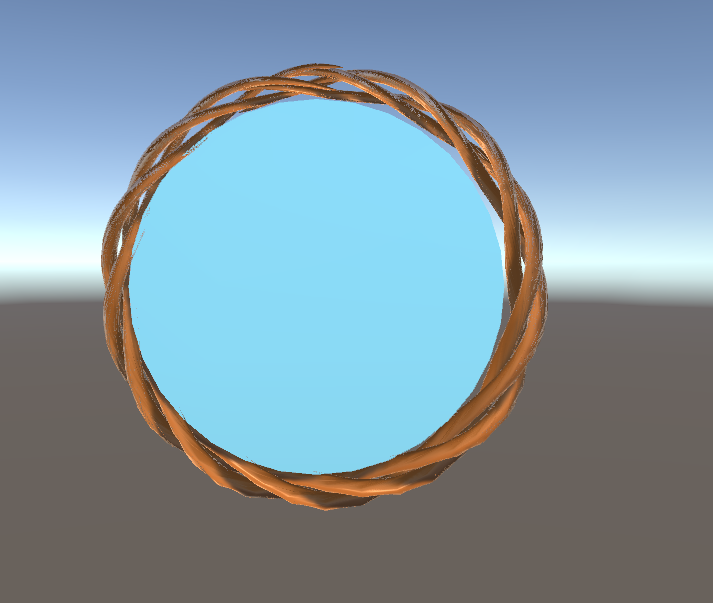
\includegraphics[scale = 0.3]{Mirror}
				\caption{A mirror.}
				\label{fig:mirror}
			\end{figure}
			
			As mentioned before in the user activities, the mirror's outer
			frame will become brightly yellow when that mirror is selected.
			A selected mirror is shown in figure \ref{fig:selectedmirror}.
			\begin{figure}[!ht]
				\centering
				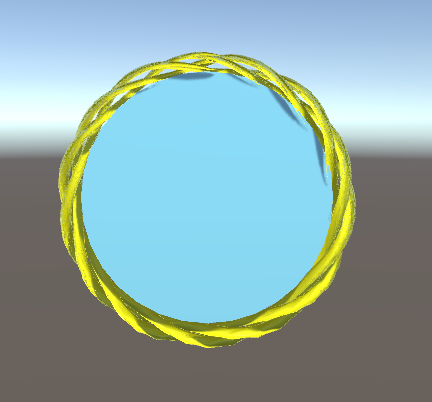
\includegraphics[scale = 0.3]{SelectedMirror}
				\caption{A selected mirror.}
				\label{fig:selectedmirror}
			\end{figure}
			
		\subsection{Wall} \label{ssec:wall}
			The wall is the main obstacle in the game. It blocks incoming
			laser beams completely. Walls are used in levels to make it 
			harder for one player to reflect a laser beam coming from
			an emitter to the target. The first few levels mainly use walls
			to create paths that the laser beam has to go through, later
			levels use not only walls, but also other game objects. A wall
			is shown in \ref{fig:wall}.
			\begin{figure}[!ht]
				\centering
				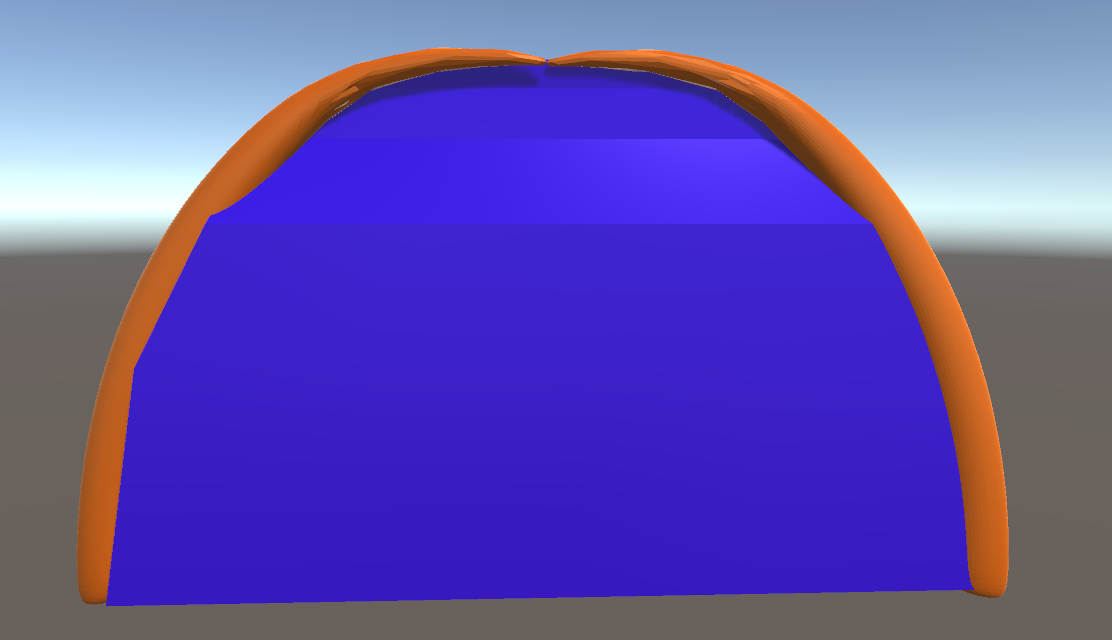
\includegraphics[scale = 0.5]{Wall}
				\caption{A wall.}
				\label{fig:wall}
			\end{figure}
			
		\subsection{Emitter} \label{ssec:emitter}
			The emitter is the most important aspect of the entire game.
			It is the only "true" source of a laser beam (although game
			elements like the beam splitter can also create beams, these
			elements always require input in the form of another laser
			beam; the emitter does not have that problem, hence it is a "true"
			source). In the early levels, players only move and rotate mirrors
			to guide a laser beam from the emitter to the target, while in the
			later levels beams have to be guided towards other game elements
			(like the beam splitter, for example) in order to complete the
			level. It is possible to have multiple emitters in a single level,
			and later levels use this to create more complex puzzles.
			What the emitter looks like exactly is shown in figure 
			\ref{fig:emitter}. Also shown here is a laser beam
			coming from the emitter. The laser beam is colored red per 
			standard. There are game objects that can change the coloring of 
			the beam, these will also be described in this part of the report.
			\begin{figure}[!ht]
				\centering
				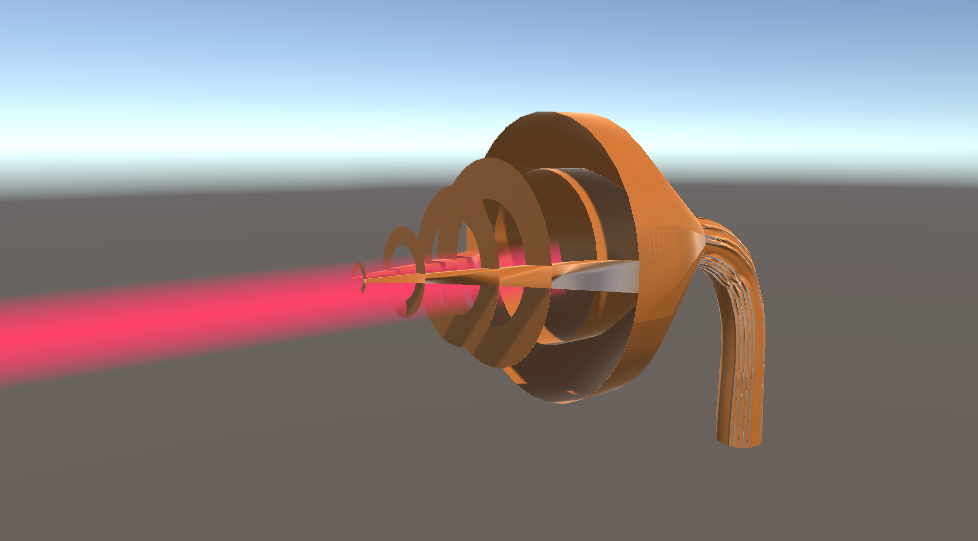
\includegraphics[scale = 0.25]{Emitter}
				\caption{The emitter.}
				\label{fig:emitter}
			\end{figure}
			
		\subsection{Elevator} \label{ssec:elevator}
			The elevator is a game object that uses mirrors to elevate laser beams
			to a new height. This then allows laser beams to pass over walls that 
			stand on the ground. Therefore, elevators can function as a bridge over
			walls. An elevator is depicted in \ref{fig:elevator}. Both the upper and 
			lower plate have a mirror (represented on the bottom plate as a light 
			blue plate), which reflects laser beams.
			\begin{figure}[!ht]
				\centering
				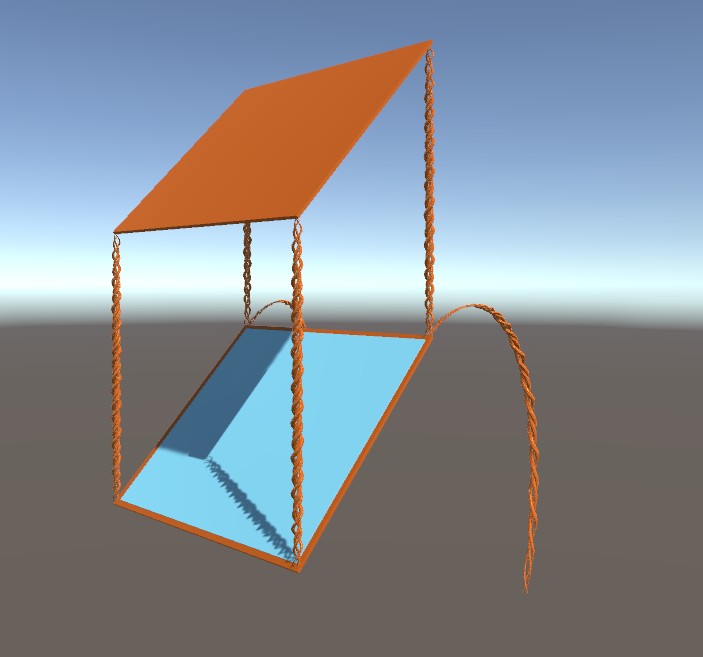
\includegraphics[scale = 0.3]{Elevator}
				\caption{An elevator}
				\label{fig:elevator}
			\end{figure}
			
		\subsection{Checkpoint}
			The checkpoint is a very important game object. Once a checkpoint is
			hit, it is registered that the checkpoint has been hit until the
			laser beam hitting it is no longer aimed towards it. In order to
			proceed to the next level, one needs to hit all the checkpoints
			in the level as well as all the targets. Checkpoints do not require
			that the laser beam has any specific color in order for them to register
			that they have been hit. The checkpoints also allow lasers to pass
			through them. Checkpoints have been added mainly to prevent sequence
			breaking of a level (sequence breaking is a term used in video games
			for being able to get to a goal using a different route than you were
			supposed to, often making it far easier than it should be. Gamers making
			use of this "break the sequence" of actions in the game, hence the term).
			An image of a checkpoint is shown in TODO
			%TODO: IMAGE CHECKPOINT.
			
		\subsection{Portal} \label{ssec:portal}
			The portal is a more advanced game object. It allows light that travels 
			into it to travel out of the portal it is linked to, and vice versa. This
			allows puzzles to contain targets that cannot be hit by just reflecting
			laser beams from the emitters by mirrors (as the laser beams have to
			travel through a portal in order to be able to hit the target),
			therefore forcing the players to redirect laser beams to portals.
			A portal is depicted in \ref{fig:portal}. It looks like a 
			recolored mirror. It has one black side and one green side. The 
			black side is the side that allows laser beams to travel through 
			it to the portal linked to it. The green side blocks laser beams completely.
			\begin{figure}[!ht]
				\centering
				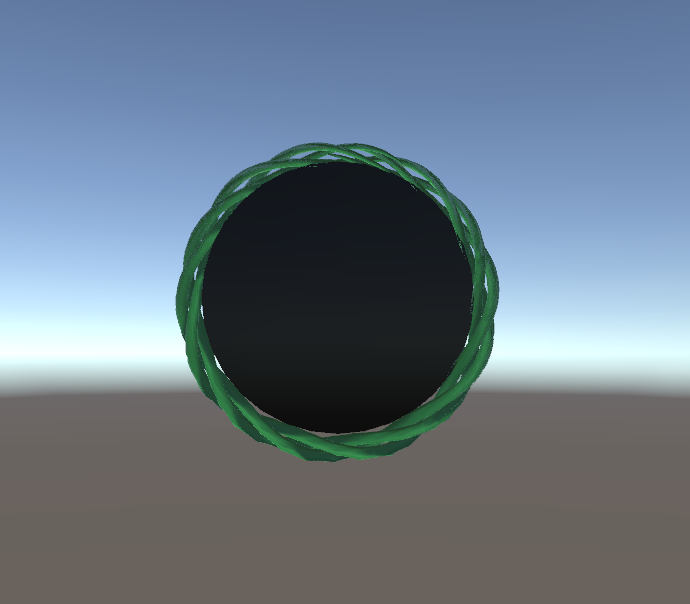
\includegraphics[scale = 0.3]{Portal}
				\caption{The portal.}
				\label{fig:portal}
			\end{figure}
			
		\subsection{Lens splitter} \label{ssec:splitter}
			The lens splitter is another advanced game object. It splits incoming
			laser beams into two, creating two separate laser beams that each go
			a different way. This allows creation of another laser beam without
			another emitter, which allows hitting of multiple targets, for
			example. A lens splitter is depicted in \ref{fig:lenssplitter}. As
			can be seen, it has two lenses (to focus the laser beam to the crystal)
			and a crystal (to split the incoming beam). The incoming beam has to hit
			the outer lens, and the outgoing beams will be emitted from the outer
			points of the crystal.
			\begin{figure}[!ht]
				\centering
				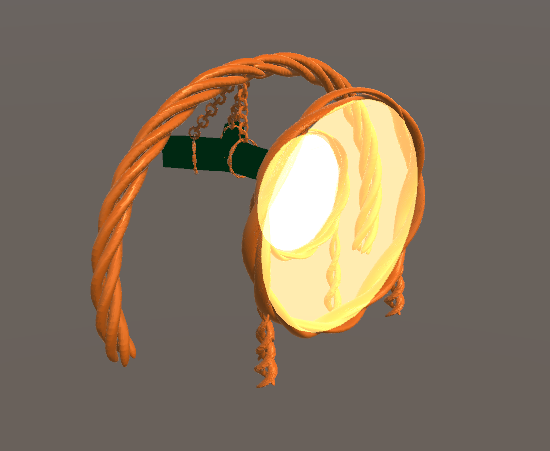
\includegraphics[scale = 0.3]{LensSplitter}
				\caption{The lens splitter.}
				\label{fig:lenssplitter}
			\end{figure}
			
		\subsection{Planned game objects that didn't make it} \label{ssec:planned}
			There were some ideas for game objects that did not make the
			final cut. For example, there were plans to use AND- and OR-gates
			that received beams as input and emitted beams when enough input
			was given (this would be at least one beam for the OR-gate, and
			at least two for the AND-gate, while these gates would then emit
			a single beam as output). These were the first logic gates that
			we thought about, and later ideas included XOR and NO-XOR gates
			(gates that would only emit a laser beam when hit by an odd or 
			even amount of beams, respectively). There was (and still is) 
			code that manages the behavior of AND- and OR-gates, however, 
			there were no models, and after talking
			about them with our coach after the first demo, we concluded that
			these objects would not add much more to the game, and as such,
			development on them was scrapped.
			
			Another idea that was eventually scrapped was the inclusion of
			switches that would be triggered by aiming a beam on them, which
			would then cause a wall linked to the switch to become transparent,
			allowing light to pass through it. This would cause players to
			collaborate to aim a beam to the switch, and then to aim another
			beam through the transparent wall. However, no models nor scripts
			were developed for this functionality, and the idea was eventually
			scrapped.
			
	\section{Level design} \label{sec:leveldesign}
		Levels are designed to be simple at first, requiring little collaboration,
		while getting progressively harder, as well as introducing more and more
		game objects. The following sections describe the level categories as
		well as which game elements these levels introduce to the player.

		\subsection{Levels 1 to 5: the basic tutorial levels} \label{ssec:basiclevels}
			The first five levels introduce the player to the most basic game
			elements that the game has to offer. These include walls, mirrors,
			and the laser target. Mechanics introduced and explained in these
			levels are: walls block incoming laser beams, mirrors reflect
			incoming laser beams, one needs to hit all laser targets in order
			to proceed to the next level, and the color of the emitted laser
			beam should correspond to the color of the crystal it is hit with.
			
		\subsection{Levels 6 to 15: the easy levels} \label{ssec: easylevels}
			These levels serve to introduce the player to slightly more advanced
			game objects and their functions. As such, they introduce elevators
			and lens splitters, as well as checkpoints. Game mechanics introduced
			in these levels are: elevators allow a laser beam to pass over objects,
			lens splitters create two beams from one, and all checkpoints in a
			map need to be hit before one can proceed to the next level. The
			levels that introduce these features are designed to be impossible
			to complete without making use of these new features (this is an
			inherent function of the checkpoints, as one can only advance to the
			next level if all checkpoints have been hit, thus making use of
			the checkpoints). For example, when introducing the elevator, the
			laser target is in a closed off area and can only be reached by
			using an elevator to elevate the beam, before lowering the beam using
			another elevator, when the beam has reached the closed area.
			
		\subsection{Levels 16 to 25: the advanced levels}
			These levels introduce the players to the last game object remaining:
			the portal. Also, the levels are a lot more difficult and require
			far more cooperation than the easy levels, from both the local
			and the remote players. Game mechanics introduced in these levels
			are: portals allow beams to travel to places normally unreachable.